\documentclass{article}

\usepackage{neurips_2026}
\usepackage[utf8]{inputenc}
\usepackage[T1]{fontenc}
\usepackage{hyperref}
\usepackage{url}
\usepackage{booktabs}
\usepackage{graphicx}
\usepackage{amsmath}
\usepackage{xcolor}
\usepackage[normalem]{ulem}
\usepackage{microtype}

\graphicspath{{figures/}}
\newcommand{\TODO}[1]{\textcolor{red}{\textbf{TODO: #1}}}
\newcommand{\pp}{\,\mathrm{pp}}

\title{What Should a Joint-Embedding Predictor Predict?\\
Target Composition, Context Loss, and Equity in Medical Image SSL}

\author{}

\begin{document}

\maketitle

\begin{abstract}
Masking policy is an under-audited design choice in medical self-supervision.
We study patch-level I-JEPA pretraining for glaucoma classification from
optical coherence tomography (OCT). We found no prior report of the following
medical-imaging consequence of stock I-JEPA batching: variable-length context
masks are truncated to the batch minimum by retaining a row-major prefix,
systematically deleting lower image rows. In our rectangle-based arms this
removes 31--36\% of sampled context and leaves up to 11.02\% of slices with no
retinal anatomy delivered to the encoder. Across four epoch-50 arms, frozen
probe AUC is non-monotonic in target anatomy purity
(31.6\%$\rightarrow$0.8641, 39.7\%$\rightarrow$0.8740,
43.2\%$\rightarrow$0.8761, 97.5\%$\rightarrow$0.8654). The near-pure arm's
predictor error rises 2.76$\times$ while its relative reliance on anatomy
context falls, supporting predictor collapse rather than anatomy starvation.
Post-hoc equity analysis finds Black patients worst served in all 18 valid
probes; racial AUC gaps vary 1.97$\times$, whereas the severe-to-mild disease
gap remains 0.1286--0.1394. These are single-seed, observational results:
18 probes derive from six pretraining trajectories, the test split was consulted
during earlier development so all findings are exploratory rather than
confirmatory, and we do not claim that anatomy-shaped targets outperform
rectangles.
\end{abstract}

\section{Introduction}

Masked and predictive self-supervision learns visual representations by
withholding part of an image and predicting pixels, tokens, or latent
representations \citep{he2022mae,bao2022beit,assran2023ijepa}. The masking
policy determines both what supervision is presented and what evidence remains
visible. This choice is especially consequential in retinal OCT, where anatomy
occupies a narrow band within many B-scans.

We audit I-JEPA \citep{assran2023ijepa} on the FairVision glaucoma cohort
\citep{luo2024fairvision}. The programme began with the hypothesis that
connected anatomy-shaped targets would beat anatomy-guided rectangles. The
evidence rejects that framing: anatomy is ahead by 0.0054 at epoch 30, but the
direction reverses by $-0.0107$ at epoch 50, and the early comparison uses
different guide caches. We therefore study the more defensible question:
\emph{what effective prediction problem does a mask policy create after
collation?}

Our contributions are:
\begin{itemize}
  \item We trace a spatially biased context-erasure failure to stock-style
  batch-minimum prefix truncation and quantify its batch-size dependence.
  \item We measure target and delivered-context composition, finding an
  observational, non-monotonic purity--AUC relationship rather than a universal
  purity optimum.
  \item We diagnose the near-pure arm's failure as predictor collapse, while
  refuting the simpler anatomy-starvation explanation.
  \item We show consistent racial ordering across saved probes and a
  policy-invariant mild-disease penalty, with statistical and independence
  limits stated explicitly.
\end{itemize}

\section{Background and related work}

\paragraph{Joint-embedding prediction.}
I-JEPA predicts target-encoder representations from a masked context view
\citep{assran2023ijepa}. Subsequent work studies representation collapse and
target ordering \citep{mo2024cjepa,he2025dseqjepa}, but we found no prior
report of the spatially biased context-erasure mode examined here. Our claim is
search-qualified: we report a medical-imaging consequence of released
I-JEPA-style mask batching for which we found no prior report, not a defect
unique to our anatomy-guided code.

\paragraph{Semantic and anatomical masking.}
Attention-guided and reconstruction-guided methods establish that target
content matters \citep{kakogeorgiou2022attmask,li2024anatomask}.
Ceballos Arroyo et al.\ use a pretrained segmenter to guide masked
autoencoding in medical images \citep{ceballosarroyo2026anatomymae}; related
anatomical masking also predates this study \citep{huang2025amap}. We therefore
do not claim the first anatomy-guided medical masking method. Our narrower
contribution is an OCT/I-JEPA audit that measures target purity, delivered
context, predictor health, and trajectory reversal.

\paragraph{Ophthalmic equity.}
Medical models can encode demographic signals and exhibit subgroup disparities
\citep{gichoya2022race,jin2024fairmedfm}. FairVision was designed to support
equity analysis in ophthalmic AI \citep{luo2024fairvision}. We use its released
race and disease-severity attributes, but treat repeated probes from the same
encoder as non-independent.

\section{Experimental setup}

\paragraph{Data and permitted use.}
We use the released FairVision glaucoma cohort. Its split contains 6,000
training, 1,000 validation, and 3,000 test OCT volumes. Each
\texttt{oct\_bscans} array is a
$200\times200\times200$ uint8 B-scan stack. Evaluation samples 100 of the 200
B-scans per volume. The test set has 1,466 positive and 1,534 negative volumes.
The data license is CC BY-NC-ND 4.0 and permits non-commercial research, not
clinical use.

\paragraph{Encoder and probing.}
We use patch-level I-JEPA with a ViT-B/16 encoder
\citep{dosovitskiy2021vit}. Slices are processed on a $16\times16$ patch grid.
Unless stated otherwise, evaluation freezes the encoder, mean-pools patch
features, and fits a linear glaucoma head with probe seed 42. Every masking arm
descends from the same epoch-25 checkpoint, whose test AUC is 0.8487. This
shared ancestor improves comparability but does not replace pretraining-seed
replication.

\paragraph{Mask policies and measurements.}
Random uses standard multiblock rectangles; oracle places rectangles using a
hand-crafted retinal band; envelope places rectangles using frozen MIRAGE
segmentation \citep{morano2025mirage}; COVER greedily places rectangles while
enforcing an anatomy-visibility floor; and blob uses connected, near-pure
anatomy targets. For each slice we measure anatomy recall by targets, target
purity, anatomy retained in delivered context, target/context budgets, and the
zero-anatomy context rate.

\section{Spatially biased context erasure}

\subsection{Mechanism}

The defect is a three-link causal chain in the mask collator:
\begin{verbatim}
self.height = input_size[0] // patch_size
self.width = input_size[1] // patch_size
indices.append(r * self.width + c)
masks_enc[e].append(
    torch.tensor(sorted(best_indices), dtype=torch.long)
)
min_len = min(t.numel() for t in group)
torch.stack([t[:min_len] for t in group], dim=0)
\end{verbatim}
First, $r\times\texttt{width}+c$ is row-major: every index in a lower image
row exceeds every index in a higher row. Second, encoder masks are explicitly
sorted ascending before storage. Third,
\texttt{\_truncate\_and\_stack} retains \texttt{t[:min\_len]}. It therefore
keeps the smallest indices---the top rows---and discards the largest
indices---the bottom rows. The row-major ascending ordering, created by
\texttt{\_block\_to\_indices} and redundantly re-enforced by \texttt{sorted()}
at encoder storage, is what makes this excision deterministic and spatially
systematic rather than a random subset.
In OCT B-scans the retinal band occupies a limited vertical extent, so this is
a systematic anatomical excision, not benign padding
(Figure~\ref{fig:excision}).

\begin{figure}[t]
\centering
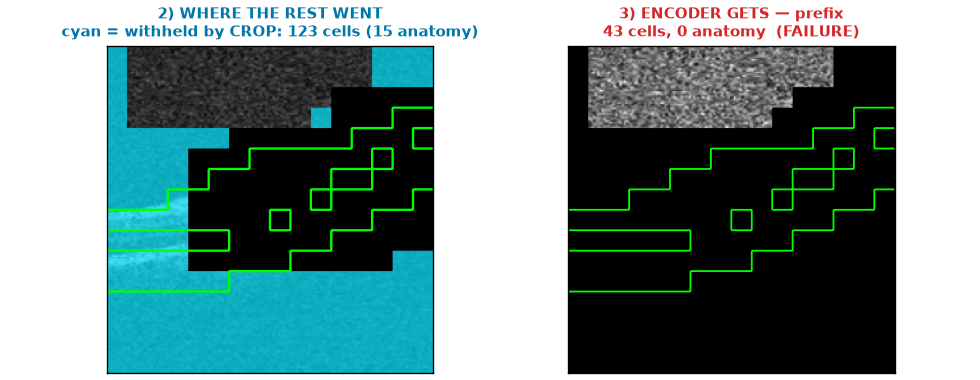
\includegraphics[width=\linewidth]{fig1b_context_excision.png}
\caption{Measured retained-versus-discarded encoder context for a stored
failing slice. Cyan marks 123 non-target cells not delivered to the encoder,
including 15 anatomy cells; the encoder receives 43 smallest-index cells from
the top rows and zero anatomy. The total withheld count includes pre-collation
context selection as well as batch truncation. Green traces the retinal guide.
This panel is cropped from the stored diagnostic image.}
\label{fig:excision}
\end{figure}

This is a faithful port of released upstream behavior (I-JEPA commit
\texttt{52c1ae95d05f743e000e8f10a1f3a79b10cff048}, mask-collator lines
145--175), not a local defect introduced by our anatomy code. We are not aware
of a prior report of this failure mode. In our rectangle arms at batch size 64
it removes 31--36\% of sampled context, including for plain random masks.

The proof above applies only to encoder/context masks. Predictor masks are
stored without the \texttt{sorted()} call and follow a separate, more
aggressive path: one global minimum is taken across every predictor group and
sample before retaining \texttt{t[:global\_min\_pred]}. We therefore make no
claim about the spatial character of predictor-mask truncation.

\begin{figure}[t]
\centering
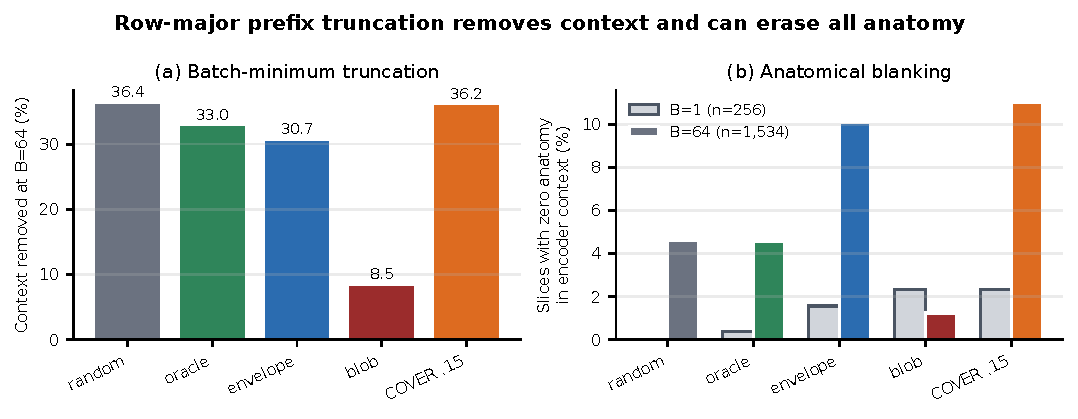
\includegraphics[width=\linewidth]{fig1_crop_defect.pdf}
\caption{Batch-size audit of prefix truncation. Rectangle policies lose
31--36\% of sampled context at $B=64$. Zero-anatomy context increases from
$B=1$ to $B=64$: random 0.00$\rightarrow$4.63\%, envelope
1.56$\rightarrow$10.10\%, and COVER $f=.15$ 2.34$\rightarrow$11.02\%. The
audits use $n=256$ and $n=1{,}534$ slices, respectively, and are separate
samples rather than a paired intervention. The independent $n=6{,}137$ pass of
Table~\ref{tab:composition} puts the same $B=64$ rates at 3.68\% and 8.07\%;
we report both passes rather than pooling them.}
\label{fig:crop}
\end{figure}

\subsection{Failure accounting}

The effect is anatomically consequential
(Figures~\ref{fig:excision}--\ref{fig:crop}). In one
failing slice, all 256 patches balance exactly as 90 targets, 123 withheld
patches, and 43 patches delivered to the encoder. Its 65 anatomy patches
balance as 50 targeted and 15 withheld, leaving zero anatomy visible. The
withheld count includes pre-collation context sampling as well as batch
truncation, so it is not attributed to truncation alone.

Repeated draws show that this is not an intrinsic ``bad slice'' property:
0\% of slices are always blank, and 52.0\% are never blank versus 44.6\%
expected under 12 independent draws at the aggregate 6.5104\% blank rate. The
failure varies across draws; the 12-draw audit found no fixed always-blank
subset, although blanking risk remains concentrated in some slices.

\section{Target composition and downstream quality}

\paragraph{The hypothesis we started from.}
Anatomy is where the diagnostic information is, and the predictor agrees with
that intuition. Per removed context token, anatomy is worth 3.9--6.6$\times$
more to the predictor than background across every healthy checkpoint we
measured (Figure~\ref{fig:background}a), and region-restricted probes order the
same way, with anatomy-only pooling above background-only pooling in all four
arms (Figure~\ref{fig:background}b). The natural design response is to spend
the masking budget on anatomy, and our policies do so progressively: random
rectangles place 31.6\% of target cells on anatomy, oracle 39.7\%, COVER
40.9\%, envelope 43.2\%, and blob 97.5\%.

\begin{table}[t]
\centering
\scriptsize
\setlength{\tabcolsep}{2.6pt}
\caption{Post-collation composition. Values are percentages except context
cell counts and AUC. AUC uses the standard 100-slice, seed-42 frozen mean-pool
linear protocol. Random, oracle, COVER, and envelope share an $n=6{,}137$
audit; blob is a separate $n=1{,}534$ pass.}
\label{tab:composition}
\resizebox{\linewidth}{!}{%
\begin{tabular}{lrrrrrrrr}
\toprule
Arm & $n$ & Recall & Purity & Ctx.\ anat. & Anat.\ cells & Ctx.\ cells &
Zero anat. & ep50 AUC \\
\midrule
random & 6,137 & 53.04 & 31.58 & 26.38 & 18.25 & 69.09 & 3.68 & .8641 \\
oracle & 6,137 & 61.58 & 39.69 & 19.34 & 14.93 & 77.23 & 4.19 & .8740 \\
COVER $f=.21$ & 6,137 & 73.09 & 40.88 & 14.56 & 9.28 & 63.62 & 7.84 & -- \\
envelope & 6,137 & 77.58 & 43.19 & 11.38 & 8.63 & 76.41 & 8.07 & .8761 \\
blob & 1,534 & 82.07 & 97.50 & 6.26 & 9.97 & 160.00 & 1.24 & .8654 \\
\bottomrule
\end{tabular}}
\end{table}

\begin{figure}[t]
\centering
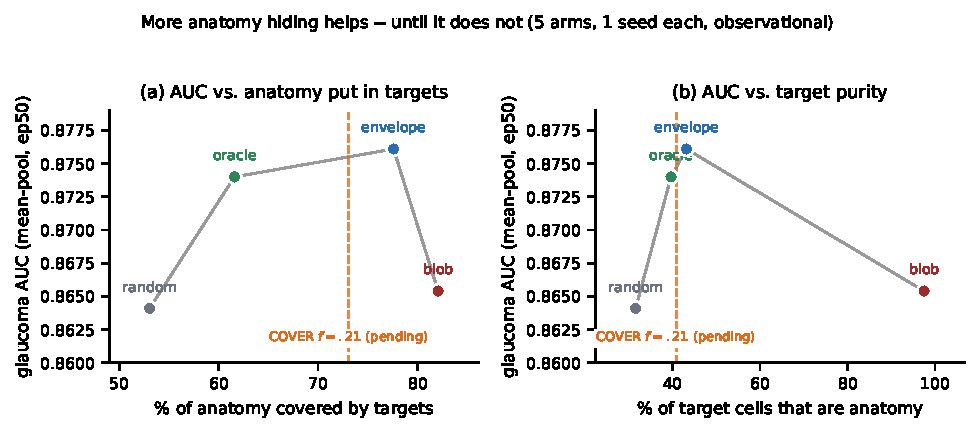
\includegraphics[width=\linewidth]{figS2_inverted_u.pdf}
\caption{Downstream AUC is non-monotonic in how much anatomy the policy puts
into targets (a) and in target purity (b). Points are the four completed arms
at epoch 50 under the frozen mean-pool protocol, one pretraining seed each; the
connecting line is a visual guide, not a fit. COVER $f{=}.21$ is shown as a
dashed marker at its measured composition because its epoch-50 probe has not
yet run. Policy changes also alter target shape, target count, context budget,
and guide source, so this is an observational dose-response hypothesis, not an
identified optimum.}
\label{fig:composition}
\end{figure}

\begin{figure}[t]
\centering
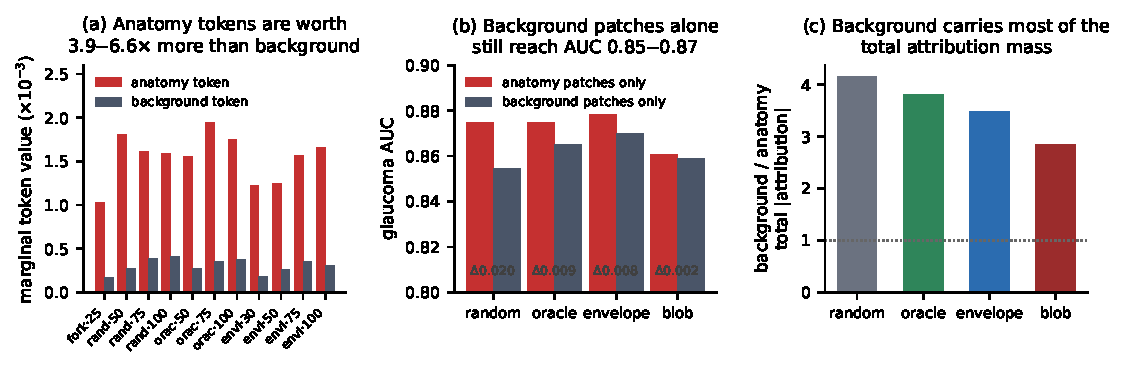
\includegraphics[width=\linewidth]{figS1_background_matters.pdf}
\caption{Anatomy is worth more per token, but background is not inert.
(a) Marginal context-token value, computed as the increase in prediction error
per removed token, for every non-collapsed checkpoint. (b) Region-restricted
frozen probes on a separate 2{,}000/600/1{,}000 volume split: background
positions alone still reach AUC 0.854--0.870, within 0.002--0.020 of anatomy
positions. (c) Exact linear attribution: background patches carry
2.8--4.2$\times$ the total absolute attribution mass of anatomy patches,
because they are far more numerous. Panels (b) and (c) use different protocols
from Table~\ref{tab:composition} and are not comparable to it in absolute
level. ViT tokens mix information globally, so ``background position'' denotes
where the token sits, not that black pixels carry signal.}
\label{fig:background}
\end{figure}

\paragraph{The hypothesis fails at the extreme.}
Table~\ref{tab:composition} separates what the sampler targets from what the
encoder receives. At epoch 50, AUC increases from 0.8641 at 31.6\% purity to
0.8740 and 0.8761 at 39.7\% and 43.2\%, then falls to 0.8654 at 97.5\%
(Figure~\ref{fig:composition}). The same reversal appears against anatomy
recall: performance improves as targets cover 53.0\%, 61.6\%, and 77.6\% of
slice anatomy, then drops at 82.1\%. Among these four confounded, single-seed
arms, the two highest observed AUCs occur at purities of 39.7\% and 43.2\%.
Because four points on one dataset move several design axes together, this
sparse comparison supports only rejection of a monotonic ``more anatomy is
always better'' rule; it does not estimate a preferred range, a dose response,
or a causal purity effect.

\paragraph{Target shape is not isolated.}
At epoch 30, the stored seed-42 probes give 0.858274 for the anatomy-shaped
encoder versus 0.853917 for envelope. A paired stratified bootstrap of those
saved predictions ($B=2{,}000$, seed 42) gives $+0.00436$ with 95\% CI
$[+0.00097,+0.00776]$ and $p=0.014$; this holds both encoders fixed and
reports test-volume uncertainty only. Envelope uses hard guides while anatomy
uses a soft-guide cache, so the arms differ in more than target shape. A
separately configured anatomy-v2/blob continuation scores $0.010679$ below
envelope at epoch 50 (0.865386 versus 0.876064); because this is not a
continuation of the epoch-30 anatomy trajectory, it is not a within-run
reversal. We therefore report both checkpoints and make no target-shape
superiority claim.

\section{Mechanism: predictor collapse}

The obvious explanation for blob's decline is too little visible anatomy, but
the accounting does not support it. Blob has the lowest anatomy fraction in context
(6.26\%), yet among the guided arms it retains the most anatomy cells on
average (9.97, versus 9.28 for COVER and 8.63 for envelope) and has the lowest
zero-anatomy rate (1.24\%). The rectangle arms deliver more anatomy still
(18.25 random, 14.93 oracle), so absolute count does not order the arms by AUC
either. Neither mean anatomy-cell count nor zero-anatomy rate alone orders the
arms by AUC; this does not rule out effects of anatomy fraction, spatial
placement, or interactions with target design.

\begin{table}[t]
\centering
\small
\caption{Within-blob predictor diagnostics. Marginal value is the prediction
error increase per removed anatomy token divided by that per removed
background-position token.}
\label{tab:collapse}
\begin{tabular}{lrr}
\toprule
Checkpoint & Full-context error & Anatomy/background value \\
\midrule
ep30 & 0.104868 & 3.529$\times$ \\
ep40 & 0.224373 & 0.998$\times$ \\
ep50 & 0.271158 & 0.830$\times$ \\
ep56 & 0.289461 & 0.737$\times$ \\
\bottomrule
\end{tabular}
\end{table}

Table~\ref{tab:collapse} gives the stronger within-arm diagnostic. Prediction
error rises 2.76$\times$ from epoch 30 to 56, while preferential reliance on
anatomy context disappears. The intervention also creates a narrower task:
blob supplies 64 target slots and 54.744 unique cells, versus 154.624 slots and
118.314 unique cells for envelope, and pads shortfalls with replacement.
Near-pure targets, connected geometry, target count, padding, and larger
context are not separately identified; jointly they are consistent with, but do
not establish, drift toward a positional or prototype-based solution.

\paragraph{Background positions are not filler.}
Figure~\ref{fig:background}(b,c) quantifies the other side of the trade. Under
the region-restricted protocol, envelope epoch-50 background-position pooling
reaches AUC 0.870075 against 0.872991 using all positions, and every arm's
background-only probe lands within 0.0203 of its anatomy-only probe. In exact
linear attribution, background patches carry 2.84--4.16$\times$ the total
absolute attribution of anatomy patches. Blob is the extreme case in both
views: it has the smallest anatomy-over-background probe gap of any arm
(0.0016, against 0.0203 for random), and it is the only arm whose background
contribution separates glaucoma better than its anatomy contribution (0.855678
versus 0.846425) despite assigning greater per-patch influence to anatomy. The
arm that concentrated targets on anatomy most aggressively ended up with the
least anatomy-specific representation. Because ViT tokens mix globally, these
results locate readable signal at background \emph{positions}; they do not
show that black pixels carry glaucoma information, and no eroded-background or
content-shuffle control has been run.

\section{A coverage floor as the balance point}

\begin{figure}[t]
\centering
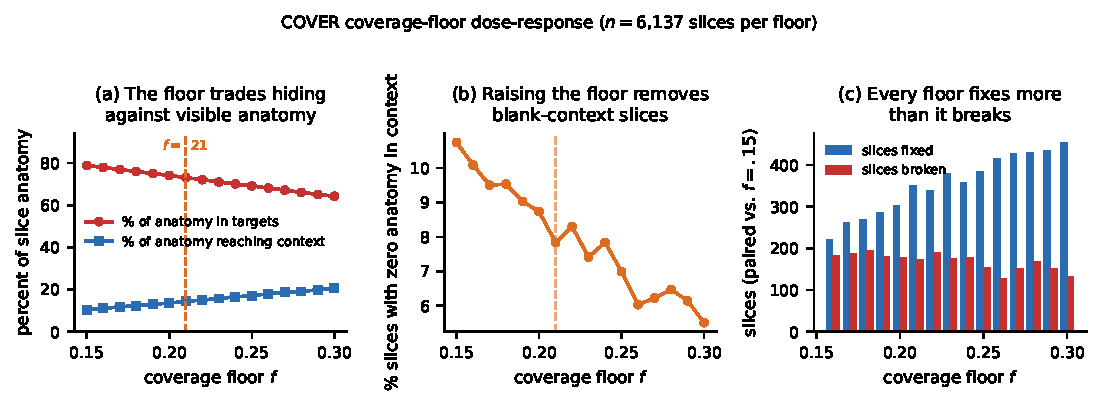
\includegraphics[width=\linewidth]{figS4_coverage_floor.pdf}
\caption{Coverage-floor dose-response, measured by resampling masks over the
same 6{,}137 slices at each floor; no pretraining is involved. (a) Raising $f$
monotonically moves anatomy out of targets and into context. (b) Blank-context
slices fall from 10.74\% to 5.51\%. (c) Against the $f{=}.15$ reference, every
higher floor repairs more slices than it breaks. This sweep identifies the
composition trade only; it is not a downstream sweep, and no AUC optimum over
$f$ is claimed.}
\label{fig:floor}
\end{figure}

The two preceding sections impose opposing constraints. Concentrating targets
on anatomy is what makes the prediction problem informative, but concentrating
them exhaustively removes the anchoring context the predictor needs, and the
arm collapses. What is required is a policy that hides most anatomy while
guaranteeing that some always survives into context.

COVER parameterises exactly this trade with one knob. A coverage floor $f$ acts
as a soft stopping rule for adding anatomy-covering blocks
(\texttt{cover\_leave\_frac}) and simultaneously as a hard per-slice constraint
that at least a fraction $f$ of anatomy cells, and at least four cells, remain
visible to the encoder (\texttt{cover\_min\_visible\_frac},
\texttt{cover\_min\_visible\_cells}). Blocks not needed for coverage are placed
as plain uniform rectangles, restricted to windows that preserve the floor.

Figure~\ref{fig:floor} sweeps $f$ from 0.15 to 0.30 over the 6{,}137-slice
audit. The trade is monotone and well behaved: anatomy placed in targets falls
from 78.84\% to 64.25\% while anatomy reaching context rises from 10.41\% to
20.69\%, and the blank-context rate falls from 10.74\% to 5.51\%. Paired
against the $f{=}.15$ reference on the same slices, every higher floor repairs
more slices than it breaks; at $f{=}.21$ the counts are 351 repaired against
173 broken ($z=-7.78$).

Two limits must be stated plainly. First, this is a mask-statistics sweep, not
a downstream sweep: it establishes that the floor controls composition in the
intended direction, and it cannot locate an AUC-optimal $f$. Second, only
$f{=}.21$ has been pretrained, and its epoch-50 probe had not completed at
submission time, so the arm appears in Table~\ref{tab:composition} and
Figure~\ref{fig:composition} without an AUC. \textbf{Assumption, flagged:} the
design rationale above predicts that a floored policy should avoid blob's
collapse while retaining envelope-like composition, but we do not yet have the
number that would test this, and nothing in this paper should be read as
reporting it. An earlier archived COVER run reached 0.8558--0.8612 over epochs
26--100, but it was executed with a different target-precision setting than the
arms it would be compared against, so its deficit is not attributable and we
exclude it.

\section{Equity and disease severity}

Saved test predictions contain no identifiers, so we join them to demographics
in deterministic test-loader order. The join is validated by exact label
reconstruction, filename order, in-volume race/gender fields, and in-volume
labels: all 3,000 labels agree in every probe directory. Four contaminated
probes are excluded below, leaving 18 valid probes drawn from six pretraining
trajectories.

\begin{figure}[t]
\centering
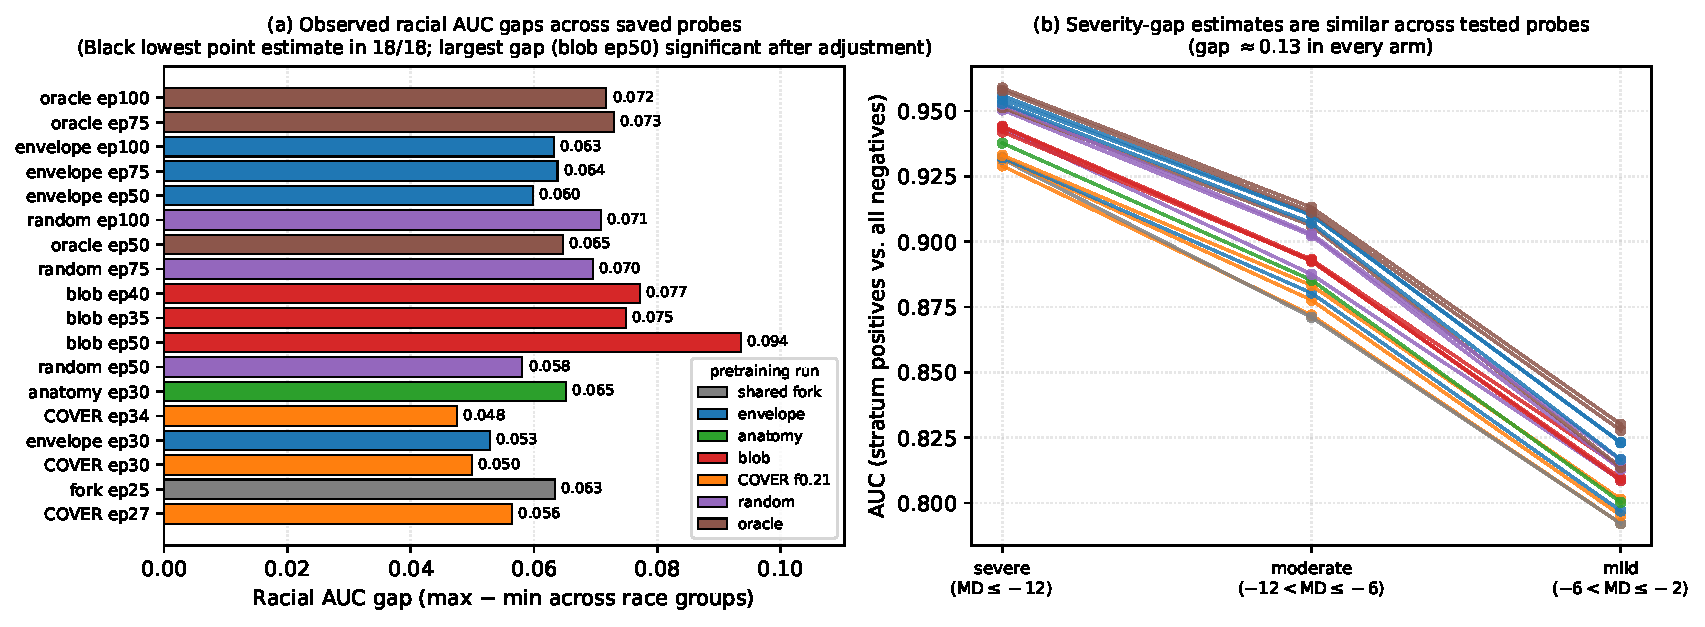
\includegraphics[width=\linewidth]{fig6_subgroup_disparity.pdf}
\caption{Subgroup results for 18 valid probes from six pretraining
trajectories. Left: racial AUC gap by arm; Black patients have the lowest AUC
in every probe. Right: each positive severity stratum is compared with the
shared negative pool because mean deviation defines the label. One individual
racial gap (blob epoch 50, Asian$-$Black) is significant after multiplicity
adjustment; the remainder are not.}
\label{fig:equity}
\end{figure}

The test split contains 2,318 white, 431 Black, and 251 Asian participants.
Black participants have the lowest AUC in 18/18 valid probes
(Figure~\ref{fig:equity}). The max--min racial gap varies 1.97$\times$, from
0.0475 for COVER epoch 34 to 0.0935 for blob epoch 50, while overall AUCs
differ by 0.0371. The rank correlation between overall AUC and racial gap is
Spearman $\rho=0.488$ (nominal $p=0.0399$), but the probes are not
independent: several are checkpoints of the same pretraining trajectory, so
this nominal significance does not license a policy-level inference and we
claim no accuracy--fairness tradeoff. One individual gap does reach
significance after multiplicity adjustment (blob epoch 50, Asian$-$Black,
0.0935, $p<0.05$); the remaining gaps do not. The most robust result is
therefore the consistency of the ordering rather than any single gap.

Mean deviation defines the FairVision glaucoma label, making within-bin AUC
undefined. We instead compare positives in each severity stratum with the same
1,534 negatives. The severe-to-mild AUC gap is 0.1286--0.1394 in every valid
probe, a spread of 0.0108. Descriptively, no tested mask policy narrows the
mild-disease penalty; with one trajectory per policy we do not test this
causally.

\section{Ablations and controls}

\paragraph{Batch size and composition.}
The $B=1\rightarrow64$ comparison in Figure~\ref{fig:crop} exercises the
collation mechanism: zero-anatomy context rises
0.00$\rightarrow$4.63\% for random,
1.56$\rightarrow$10.10\% for envelope, and
2.34$\rightarrow$11.02\% for COVER $f=.15$. The two batch settings are
separate audit samples rather than a paired intervention, so they bound the
effect without isolating it. Table~\ref{tab:composition} reports post-collation
composition observationally across arms that differ in more than purity, and
Figure~\ref{fig:composition} is the completed four-point purity sweep. A clean
COVER $f=.21$ trajectory reaches
AUC 0.8483, 0.8522, and 0.8571 at epochs 27, 30, and 34; these are checkpoints
within one run, not a cross-floor dose response. The matching epoch-50 probe
for this trajectory was still pretraining at the time of writing and is
therefore not reported.

\paragraph{Readout and region controls.}
\begin{table}[t]
\centering
\small
\setlength{\tabcolsep}{4pt}
\caption{Frozen-readout and regional controls. The regional probes use a
separate 2,000/600/1,000 train/validation/test split, so they are not directly
interchangeable with the
3,000-volume standard probes.}
\label{tab:ablations}
\begin{tabular}{lll}
\toprule
Control & Condition & Test AUC \\
\midrule
Probe head, random ep100 & attentive $d=1$ & 0.8706 \\
 & mean-pool & 0.8746 \\
\midrule
Region, random ep50 & all positions & 0.8608341 \\
 & anatomy positions & 0.8746555 \\
 & background positions & 0.8543614 \\
Region, oracle ep50 & all positions & 0.8682588 \\
 & anatomy positions & 0.8746475 \\
 & background positions & 0.8652265 \\
\midrule
Long-horizon placement & random ep100 & 0.8745809 \\
 & oracle ep100 & 0.8854852 \\
\bottomrule
\end{tabular}
\end{table}

The head ablation shows that mean pooling is not uniquely privileged: a
single-query attentive probe scores within 0.004 of it. In the separate random- and
oracle-epoch-50 regional probes, anatomy positions outperform background
positions; these are arm-specific controls, not a global regional
estimate.\footnote{The regional ablation uses separately trained probes. Its
random/oracle all-position AUCs are 0.8608341/0.8682588 with early stopping at
epochs 43/42, whereas the composition table uses standard mean-pool AUCs
0.8640971/0.8740299 stopped at epochs 46/47. Absolute AUCs across the two
protocols are not interchangeable.} The epoch-100 oracle/random difference is a
descriptive point estimate consistent with anatomical placement helping, but
with one trajectory per policy it does not identify a causal policy effect.

\section{Limitations and confound ledger}

These limitations bound every contribution.
\begin{enumerate}
  \item There is one pretraining seed per policy and no pretraining-seed
  replication anywhere in the programme. The 18 valid subgroup probes arise
  from only six pretraining trajectories and are non-independent, since several
  are checkpoints of the same run. The epoch-30 interval is a paired bootstrap
  over test volumes with both encoders held fixed, not a seed-variance
  estimate. The random/oracle epoch-50 mean-pool encoders were produced on
  another machine and reference checkpoints that are unavailable locally, so
  their arms cannot be locally re-probed or extended to seed replication.
  \item The anatomy/envelope epoch-30 comparison differs in continuation
  history and uses soft versus hard MIRAGE guide caches. At epoch 50, guide,
  geometry, hidden fraction, target count, padding, and context budget move
  together; the sign reversal is not a clean shape ablation.
  \item Four earlier COVER-random probes are retracted and excluded: their run
  used \texttt{enc\_truncate: window} and \texttt{amp\_target: true}. They
  cannot be pooled with the clean COVER $f=.21$ trajectory.
  \item Blob composition uses $n=1{,}534$, whereas the other composition rows
  use $n=6{,}137$. The purity analysis has only four completed AUC points on
  one dataset, so it cannot establish an optimum.
  \item Predictor collapse is diagnostic, not causal. Purity, target count,
  connected geometry, replacement padding, and context size change together.
  Background-only pooling concerns globally mixed background-position tokens,
  not proof of biomarkers in black pixels.
  \item Fairness estimates reuse one test split. Black ($n=431$) and Asian
  ($n=251$) groups are small; only one individual gap reaches significance
  after multiplicity adjustment (blob epoch 50, Asian$-$Black), and the
  nominally significant AUC--gap correlation pseudoreplicates checkpoints
  drawn from shared trajectories. Policy is confounded with seed and
  epoch; no accuracy--fairness tradeoff is identified.
  \item The study uses one dataset and frozen probes, with historical reuse of
  its test split and no external cohort. Results may change under end-to-end
  fine-tuning, other OCT devices, or other anatomy.
\end{enumerate}

\paragraph{Evidence still required.}
Three measurements would materially strengthen these conclusions and are not
yet available. First, every policy is represented by exactly one pretraining
trajectory; each would have to be repeated across pretraining seeds, with the
continuation rather than the probe as the unit of inference, before any policy
ranking could be treated as an effect rather than an observation.
Second, the anatomy-shaped and envelope continuations should be repeated under
a common guide cache, hidden budget, and target-count policy before any
shape comparison is attempted. Third, matched epoch-50 AUC across COVER
visibility floors is needed before the floor curve can be related to
representation quality.

\section{Conclusion}

Masking is not merely a pretraining hyperparameter: batching can silently
change its spatial meaning. In this OCT study, stock-style prefix truncation
erases lower-row context, target purity relates non-monotonically to downstream
quality, a near-pure target policy develops predictor collapse, and subgroup
ordering persists despite policy changes. Medical predictive
self-supervision should report target composition and the context actually
delivered after collation. The present evidence supports that audit standard,
not anatomy-shape superiority.

\label{endofmain}
\bibliographystyle{plainnat}
\bibliography{references}

\appendix
\label{startofappendix}

\section{Supplementary figures}

\begin{figure}[h]
\centering
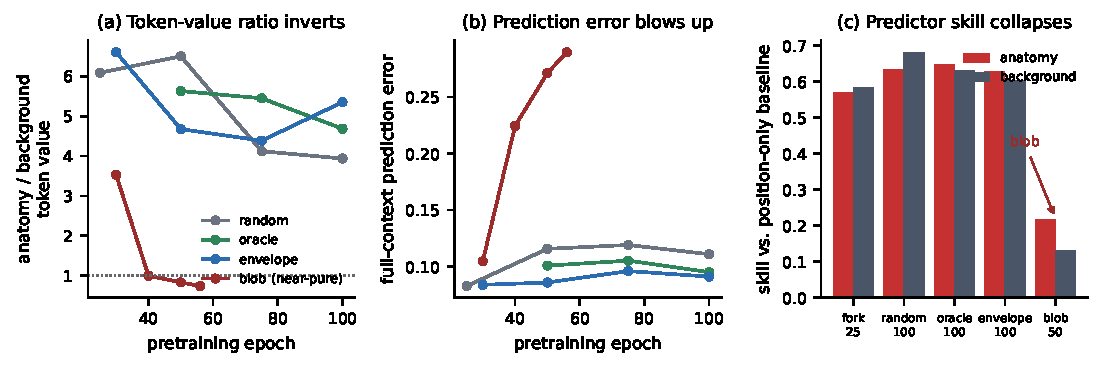
\includegraphics[width=\linewidth]{figS3_collapse_mechanism.pdf}
\caption{Within-arm collapse diagnostics for the near-pure-anatomy policy.
(a) The ratio of anatomy to background marginal token value falls below 1.0 by
epoch 40 for blob and stays there, while every other family remains between
3.9 and 6.6. (b) Full-context prediction error rises 2.76$\times$ from epoch 30
to 56 for blob and is flat elsewhere. (c) Skill relative to a position-only
baseline, measured on 108 held-out slices: blob retains 0.13 on background and
0.22 on anatomy, against 0.57--0.68 for all other checkpoints. Checkpoints are
at different epochs across families, so panel (c) compares endpoints rather
than a matched budget.}
\label{fig:collapse-fig}
\end{figure}

\begin{figure}[h]
\centering
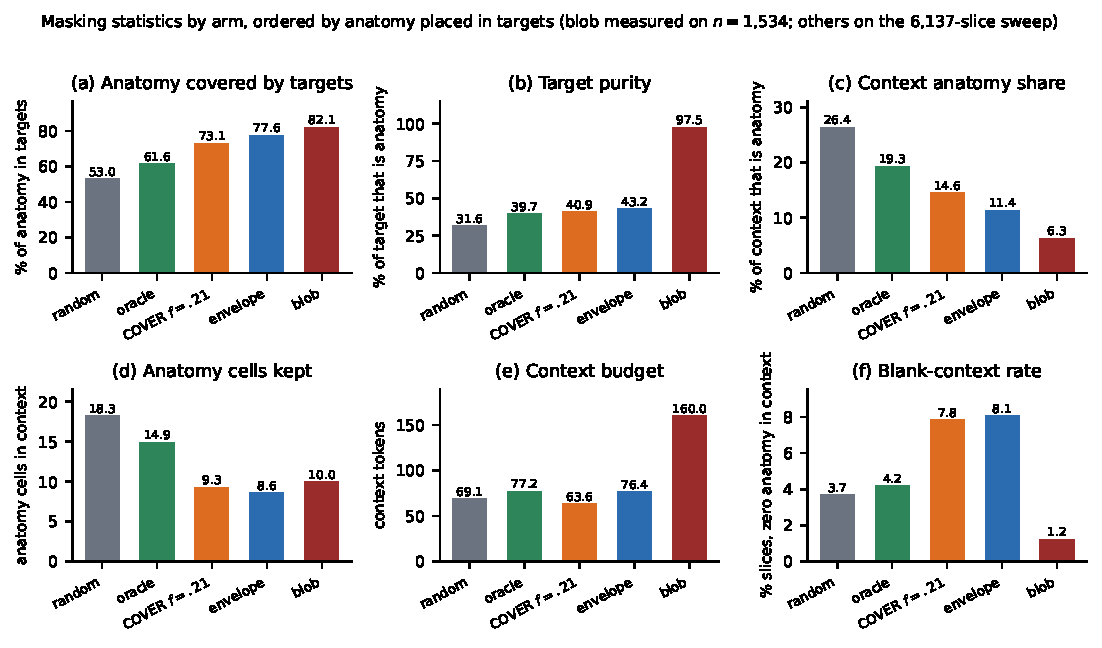
\includegraphics[width=\linewidth]{figS5_mask_statistics.pdf}
\caption{Complete post-collation masking statistics for all five arms, ordered
by the share of slice anatomy placed in targets. These are the same values
tabulated in Table~\ref{tab:composition}. Note that the two quantities most
often assumed to drive representation quality move in opposite directions
across the arms: blob has both the lowest context anatomy share (6.3\%) and the
lowest blank-context rate (1.2\%), which is why anatomy starvation does not by
itself order the arms by AUC.}
\label{fig:maskstats}
\end{figure}

\section{Planned extension: dense transfer}
\label{sec:planned}

\textbf{None of the following has been run. No result, number, or direction
reported in this section is a measurement; the section states a design and a
falsifiable prediction so that the outcome cannot be reinterpreted after the
fact.}

The audit in this paper evaluates target composition through frozen linear
probes on a single volume-level classification task. That choice isolates
representation quality from decoder capacity, but it is also the setting least
likely to reward target geometry: a volume-level label can be recovered from
pooled features that need not preserve where anatomy is. Our anatomy-shaped arm
was not better at classification, and we decline to argue that it should have
been.

Dense prediction is the setting where target geometry has a mechanism to
matter, because the pretext target and the downstream output share a coordinate
system. The planned test is therefore a transfer to layer segmentation:

\begin{enumerate}
  \item Take the terminal encoder of each pretraining arm already reported here
  --- random, oracle, COVER, envelope, and the anatomy-shaped arm --- with no
  additional pretraining, so the comparison inherits the compute-matched
  schedule and the warm-start structure documented in the experimental setup.
  \item Attach an identical lightweight decoder to every arm and fit it on an
  external labelled retinal-layer segmentation set that was not used anywhere
  in this study. Both frozen-encoder and full fine-tuning regimes are run,
  because the two answer different questions: frozen measures what the
  pretraining objective already encoded, fine-tuned measures what it made easy
  to reach.
  \item Report Dice and boundary error per layer, across the same
  race and sex strata used in the equity analysis, with cell sizes
  printed and bootstrap intervals over volumes.
\end{enumerate}

\paragraph{Stated prediction, and what would falsify it.}
We predict that the ordering observed in this paper reverses under dense
transfer: that anatomy-shaped targets, which did not help volume-level
classification, will yield higher segmentation Dice than rectangular targets at
matched compute, and that the collation repair and visibility floor introduced
here will matter more rather than less, because a truncated context removes
exactly the rows a segmentation decoder must label. The prediction is falsified
if anatomy-shaped and rectangular arms are within overlapping intervals on
Dice, which would establish that target geometry is not transferable and that
mask shape is a pretraining implementation detail rather than a
representational choice. We regard that outcome as fully possible, and it would
be reported.

\paragraph{Why it is not in this paper.}
The segmentation labels required are external to the cohort audited here and
the transfer runs have not been performed. Reporting the design without the
result is deliberate: the composition audit, the collation defect, and the
subgroup ordering stand on the evidence already presented, and none of them
depends on how the dense transfer turns out.

\end{document}
